\documentclass{article}
\usepackage{graphicx} % Required for inserting images
\usepackage[paper=a4paper]{geometry}

\title{Final Project Report}
\author{Aeysha Munawwarah}
\date{May 20 2024}

\begin{document}

\maketitle

The goal of the SURP research project is to determine if intermediate mass black holes (IMBHs) in Milky Way globular clusters (GCs) are a significant source of hypervelocity stars (HVSs) in the Milky Way. In this project, I generated samples of Hills mechanism-ejected stars and observed how the HVS population is affected by changing assumptions about the ejection model.

\section{Characterizing a Sample of Hills-ejected Stars}
\begin{figure}[h!]
\caption{\textit{A plot of Galactocentric velocity vs distance for a sample of Hills mechanism-ejected stars, ejected from the Galactic Centre by Sgr A*. In this particular run, the total number of stars was 577.}}
\centering
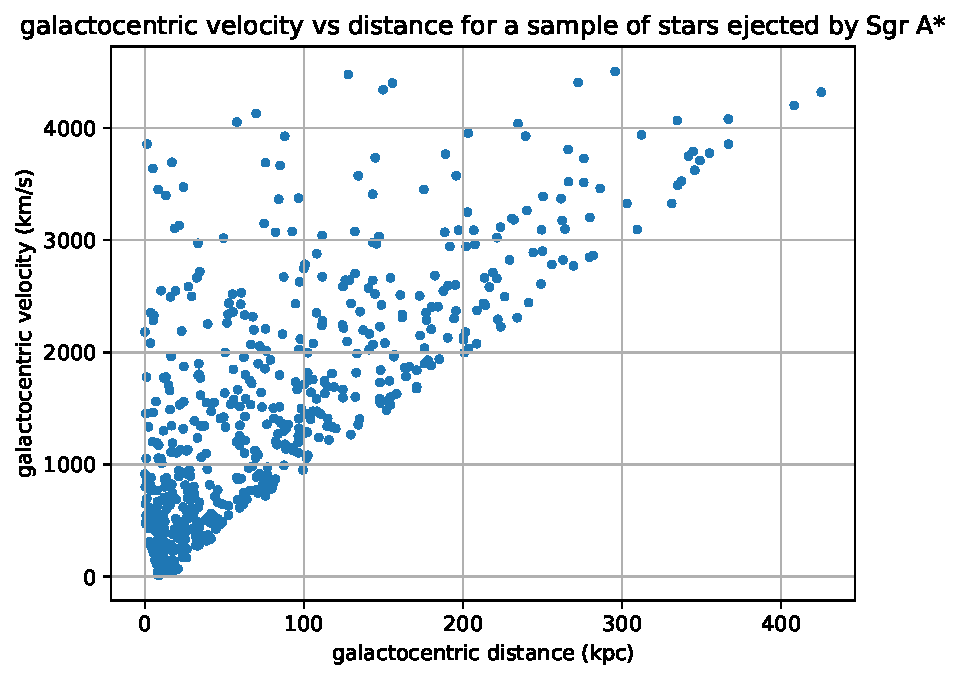
\includegraphics[width=0.65\textwidth]{GCv_vs_GCdist_1.pdf}
\end{figure}

\begin{figure}[h!]
\caption{\textit{A plot of escape velocity vs Galactocentric distance for a sample of Hills mechanism-ejected stars, ejected from the Galactic Centre by Sgr A*. In this particular run, the total number of stars was 577.}}
\centering
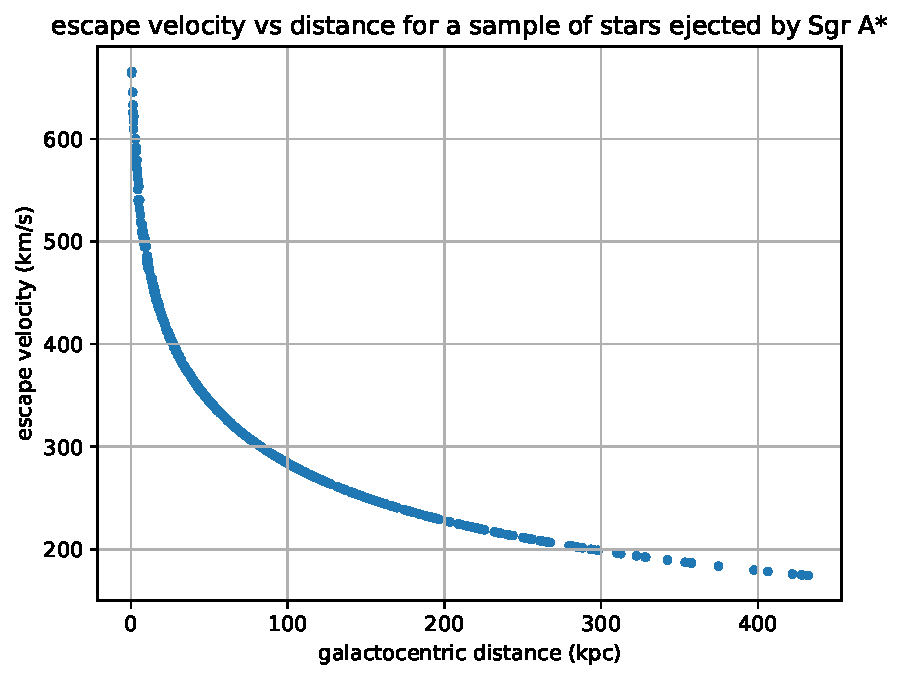
\includegraphics[width=0.6\textwidth]{Vesc_vs_GCdist.pdf}
\end{figure}

\begin{figure}[h!]
\caption{\textit{A plot of Galactocentric velocity vs distance for a sample of hypervelocity Hills mechanism-ejected stars, ejected from the Galactic Centre by Sgr A*. In this particular run, the total number of stars was 577, with a HVS population of 496.}}
\centering
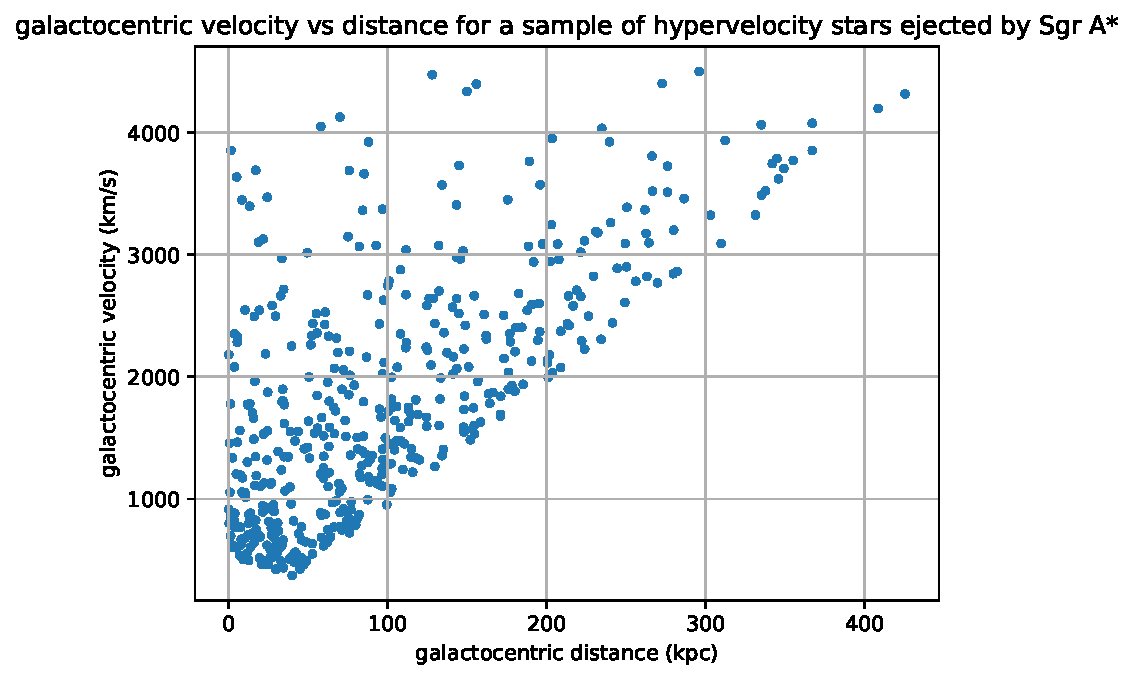
\includegraphics[width=0.8\textwidth]{GCv_vs_GCdist_hyp_1a.pdf}
\end{figure}

\begin{figure}[h!]
\caption{\textit{A plot of Galactocentric velocity vs distance for a sample of hypervelocity, Gaia DR3 detectable, Hills mechanism-ejected stars, ejected from the Galactic Centre by Sgr A*. In this particular run, the total number of stars was 577. Of that, 95 were Gaia DR3 detectable and 72 were also hypervelocity stars.}}
\centering
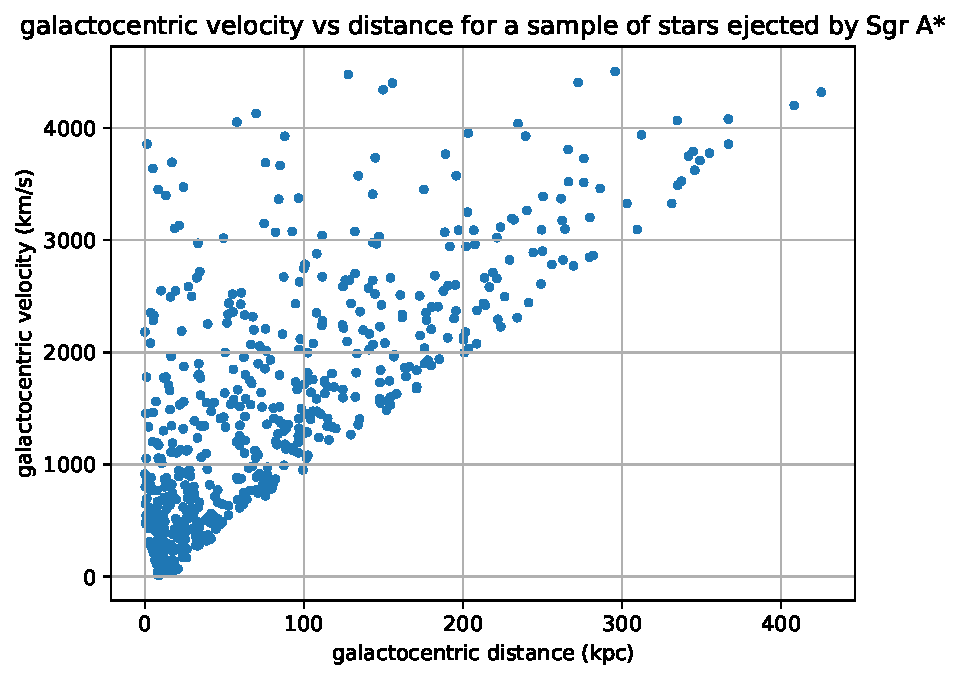
\includegraphics[width=0.65\textwidth]{GCv_vs_GCdist_1.pdf}
\end{figure}

\begin{figure}[h!]
\caption{\textit{A plot of Galactocentric velocity vs distance for a sample of hypervelocity, Hills mechanism-ejected stars, ejected from the Galactic Centre by Sgr A*. This plot compares the HVS population of the total sample (in this particular run, the total number of stars was 577, with a HVS population of 496) to the HVS population of the Gaia DR3 detectable sample (in this particular run, there were a total of 95 Gaia DR3 detectable stars, with a HVS population of 72).}}
\centering
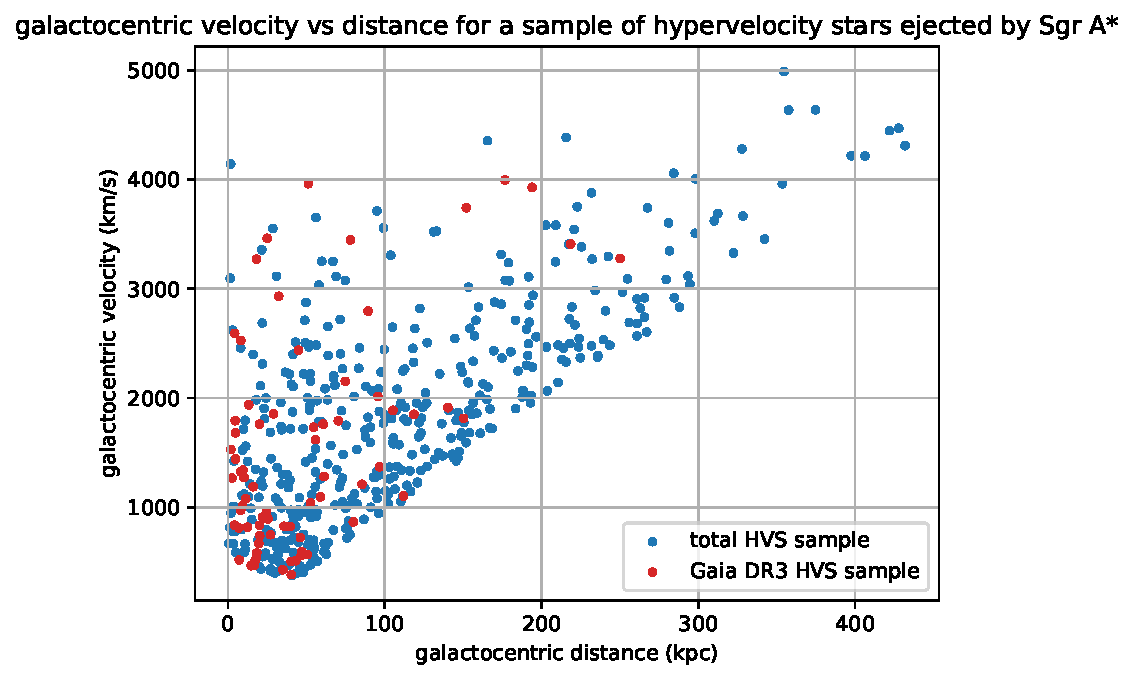
\includegraphics[width=0.8\textwidth]{GCv_vs_GCdist_hyp_1b.pdf}
\end{figure}

For this first section, I ejected, propagated and did the photometry for a sample of Hills mechanism-ejected stars. 

Assuming that the stars were ejected following interactions with Sgr A* in the Galactic Centre, I used all the default arguments for the ejection model. I then examined the data in the .fits file produced by my code and plotted the Galactocentric velocity (GCv) vs distance (GCdist) for the sample (see Figure 1). 

Looking at the plot, the ejected stars appear to be between 0 and 420 kpc away from the Galactic Centre, travelling at speeds between 0 and 5000 km/s.

I then obtained the escape velocity for each star at its position and plotted escape velocity against Galactocentric distance (see Figure 2). In this plot, it appears that with increasing distance, the escape velocity for a star decreases.

After that, I made a cut of my sample to keep only the hypervelocity stars, i.e. stars that are faster than the escape velocity. I would like to note that running the code generates a slightly different number of stars every time, and as such the HVS population also changes. 

\medskip

That being said, the total population is usually somewhere around 600, while the HVS population is around 500. Referring to Figure 3, these hypervelocity stars are mostly between 0 and 400 kpc from the Galactic Centre, travelling at speeds between 500 and 4000 km/s.

As most of these stars will be so faint and far away that they are practically impossible to detect, I then made a 'Gaia\_DR3' subsample cut to keep only the stars detectable in Gaia DR3. In this sample, there were around 70 hypervelocity stars. As seen in Figure 4, majority of these stars were between 0 and 100 kpc away from the Galactic Centre, travelling at speeds between 0 and 2500 km/s.

Figure 5 offers a direct comparison of the HVS populations of the total sample versus the Gaia DR3 subsample.

\textit{BONUS:}
In this context, escape velocity is defined as the maximum velocity that stars can have while still being bound to the Galaxy. Exceeding this would mean that a star can escape the Galaxy's gravitational grasp.
To calculate the escape velocity knowing the form of the Galactic potential, you can use an equation of the form $v_{esc} = \sqrt{2|\phi(x)|}$, where $\phi(x)$ is the gravitational potential as a function of the point $x$.

\section{The Impact of the Black Hole Mass}

\begin{figure}[htbp]
\caption{\textit{A plot of Galactocentric velocity vs distance for a sample of hypervelocity, Hills mechanism-ejected stars, ejected from a globular cluster by an intermediate-mass black hole with a mass of $4 \times 10^4 M_{\odot}$. In this particular run, the total number of stars was 342, with a HVS population of 261.}}
\centering
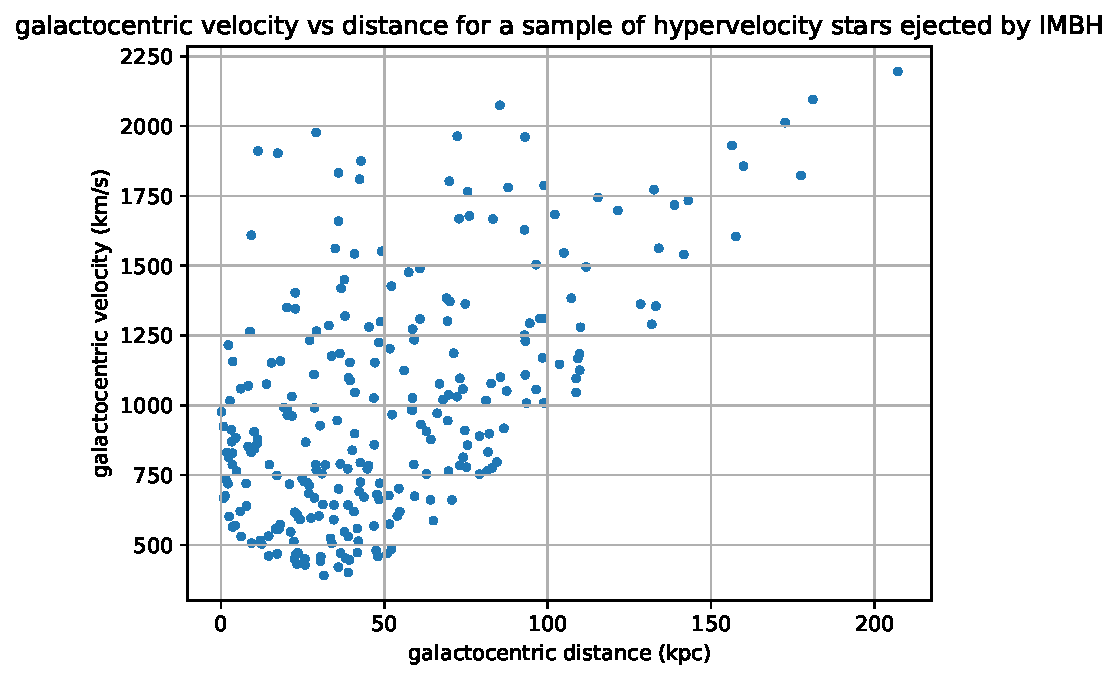
\includegraphics[width=0.8\textwidth]{GCv_vs_GCdist_hyp_2.pdf}
\end{figure}

Seeing as IMBHs are much less massive than Sgr A*, ejecting stars from IMBHs in GCs is going to be different from ejecting stars from Sgr A* in the Galactic Centre. So, in the second section, I tested the impact of black hole mass on a new catalogue of ejected stars by changing the black hole mass in the ejection model from its default value of $4 \times 10^6 M_{\odot}$ to $4 \times 10^4 M_{\odot}$. 

After following a similar process as that of section 1, I found that, in this sample, the total population was somewhere around 400, while the HVS population was around 300. Referring to Figure 6, these hypervelocity stars were mostly between 0 and 150 kpc from the Galactic Centre, travelling at speeds between 450 and 2000 km/s.

\textit{BONUS:}
In section 2.2 of the provided review article, the equation for the ejection velocity is given as: $v_{ej} = (1370 \frac{km}{s})(\frac{a}{0.1 AU})^{-1/2}(\frac{m_b}{M_{\odot}})^{1/3}(\frac{M}{4 \times 10^6 M_{\odot}})^{1/2}f_R$. In said equation, observe that $v_{ej} \propto M^{1/6}$, where $M$ is the mass of the MBH. Thus, if you reduce $M$ by a factor of $100$, $v_{ej}$ would be reduced by a factor of $100^{1/6}$.

\section{The Impact of the Initial Mass Function}

\begin{figure}[h!]
\caption{\textit{A plot of effective temperature vs mass
for a sample of hypervelocity, Hills mechanism-ejected stars, ejected from a globular cluster with kappa, the slope of its IMF, set to -2.35. In this particular run, the total number of stars was 481, with a HVS population of 440.}}
\centering
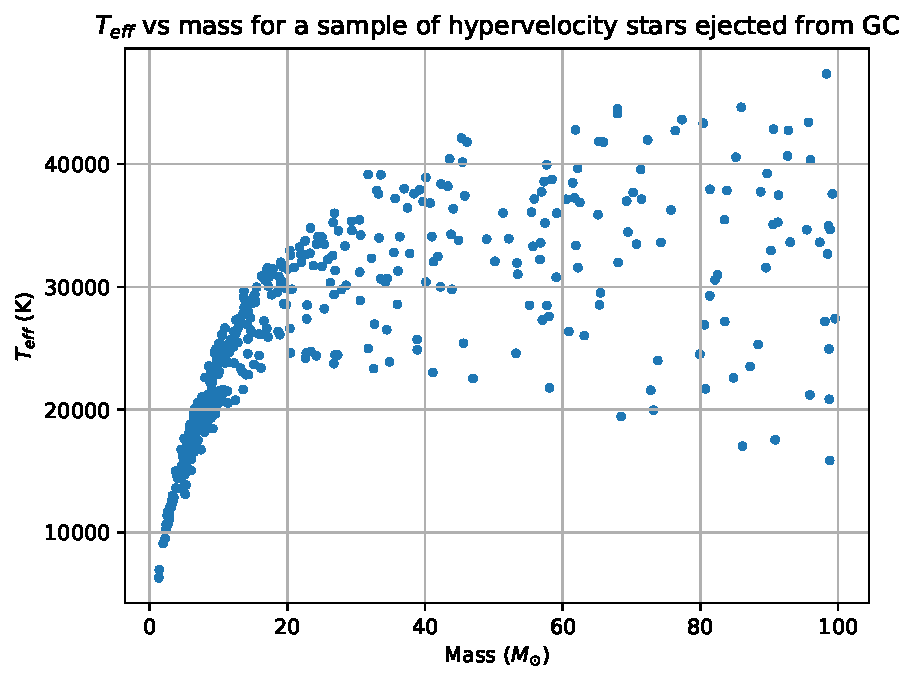
\includegraphics[width=0.7\textwidth]{Teff_vs_mass_hyp_3.pdf}
\end{figure}

The Galactic Centre and GCs also differ by way of their stellar initial mass functions. As such, in the third section, I tested the impact of the initial mass function on a new catalogue of ejected stars by changing kappa, the slope of the IMF in the ejection model, from its default value of -2.35 to -1.7.

Again, after following a similar process as that of section 1, I found that, in this sample, the total population was somewhere around 460, while the HVS population was around 430. This time, instead of Galactocentric velocity vs distance, I plotted effective temperature vs mass (see Figure 7), and found that these hypervelocity stars were between 5000 and 45000 K, with masses between 0 and 100 solar masses.

\section{The Impact of Stellar Metallicity}

\begin{figure}[h!]
\caption{\textit{A plot of effective temperature vs mass for a sample of hypervelocity, Hills mechanism-ejected stars, ejected from a globular cluster, where all ejected stars have a metallicity of -1.0. In this particular run, the total number of stars was 579, with a HVS population of 478.}}
\centering
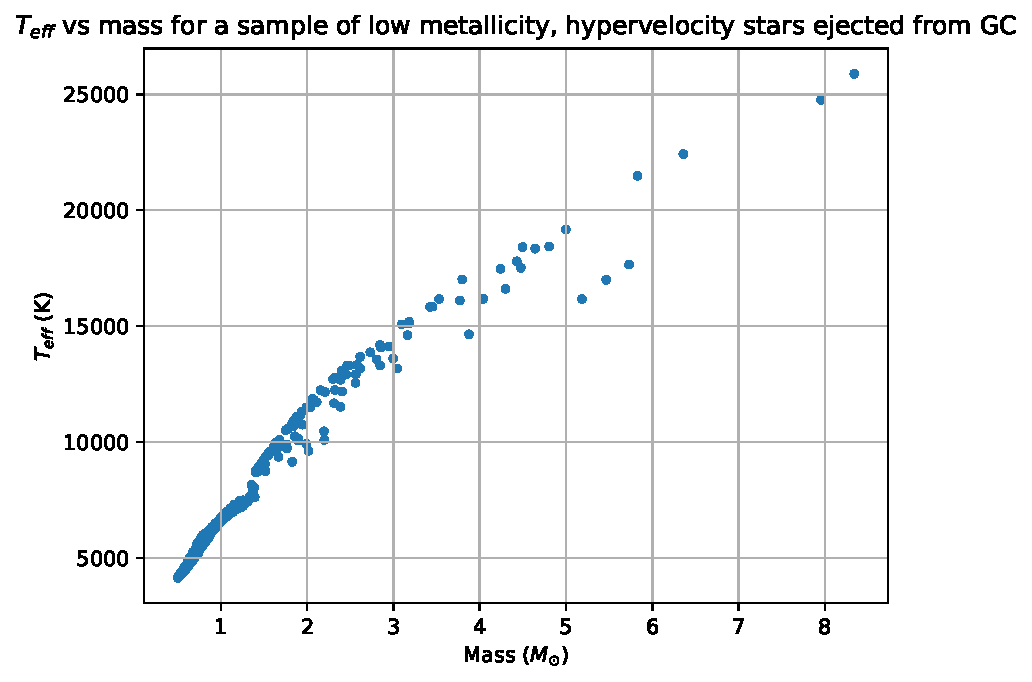
\includegraphics[width=0.75\textwidth]{Teff_vs_mass_hyp_4.pdf}
\end{figure}

Another property that sets the Galactic Centre apart from GCs is the metallicity of the ejected stars. In the ejection model, the default value assumes that all stars have the same metallicity as the Sun, when in reality, stars in the Galactic Centre have a range of metallicites and are probably on average slightly more metal-rich than the Sun. On the other hand, stars in GCs generally have lower metallicities than that of the Sun. This makes sense, as GCs stopped forming stars billions of years ago, and are thus filled with older populations of stars with lower metallicities, whereas the Galactic Centre is still actively star-forming, with younger stars.

In any case, metallicity affects the physical sizes and lifetimes of the stars, which in turn impacts their maximum flight times, maximum ejection velocities and apparent magnitudes. In the fourth section, I tested the impact of stellar metallicity on a new catalogue of ejected stars by changing the assumed metallicity in the ejection model from its default uniform distribution to all ejected stars having a metallicty of -1.0.

Once again, after following a similar process as that of section 1, I found that, in this sample, the total population was somewhere around 560, while the HVS population was around 500. Again, instead of Galactocentric velocity vs distance, I plotted effective temperature vs mass (see Figure 8), and found that these hypervelocity stars were mostly between 4500 and 20000 K, with masses between 1 and 5 solar masses.

\section{BONUS: The Impact of the Galactic Potential}

\begin{figure}[h!]
\caption{\textit{A plot of Galactocentric velocity vs distance for a sample of hypervelocity, Hills mechanism-ejected stars, ejected from the Galactic Centre by Sgr A*. Here, a different Galactic potential is implemented. In this particular run, the total number of stars was 574, with a HVS population of 427.}}
\centering
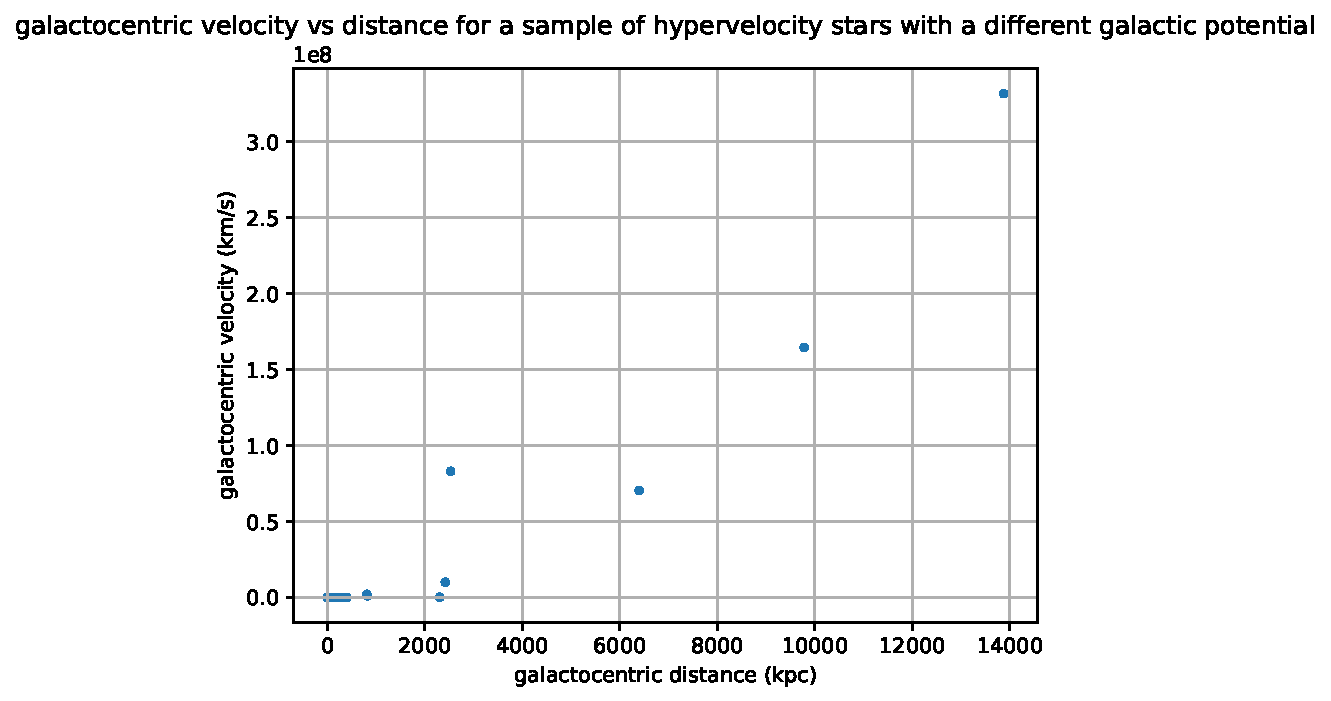
\includegraphics[width=0.9\textwidth]{GCv_vs_GCdist_hyp_5a.pdf}
\end{figure}

\begin{figure}[h!]
\caption{\textit{A plot of Galactocentric velocity vs distance for a sample of hypervelocity, Hills mechanism-ejected stars, ejected from the Galactic Centre by Sgr A*. Here, a different Galactic potential is implemented, and the mass of the halo is doubled as well. In this particular run, the total number of stars was 547, with a HVS population of 375.}}
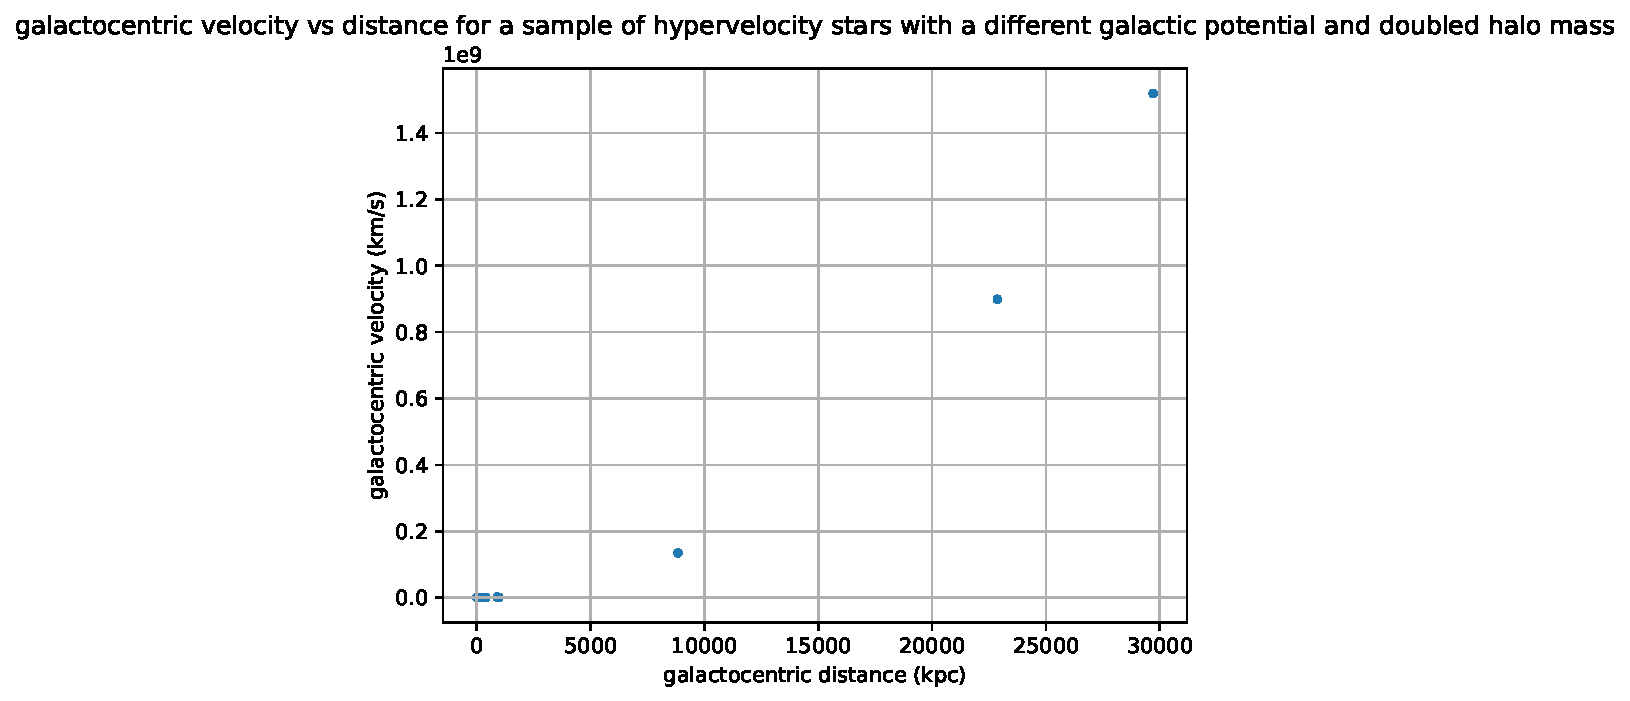
\includegraphics[width=1.1\textwidth]{GCv_vs_GCdist_hyp_5b.pdf}
\end{figure}

There is still significant uncertainty about the strength and form of the gravitational potential of the Galaxy (particularly at large distances) and this affects the HVS population. And so, in the fifth section, I tested the impact of the Galactic potential on a new catalogue of ejected stars in two cases. 

MWPotential2014 is a commonly used potential for the Galaxy, so that's what I'd used in my code up to this point. In both cases, I changed the potential to a different reasonable one using the function 

\noindent\texttt{speedystar.util.mwpotential.MWPotential()}. Then, in the second case, I also went ahead and changed the Milky Way halo mass to double its default value of $0.76 \times 10^{12} M_{\odot}$.

\vspace{1cm}

Yet again, after following a similar process as that of section 1, I found that, in the first sample, the total population was somewhere around 600, while the HVS population was around 450. I went back to plotting Galactocentric velocity vs distance (see Figure 9) and found that these hypervelocity stars were between 0 and 1500 kpc away from the Galactic Centre, travelling at speeds between 0 and $0.1 \times 10^8$ km/s. 

In the second sample, as seen in Figure 10, the total population was somewhere around 560, while the HVS population was around 400. Most of these hypervelocity stars were between 0 and 2000 kpc away from the Galactic Centre, travelling at speeds between 0 and $0.1 \times 10^8$ km/s. 

\end{document}
